\documentclass[tikz,border=8pt]{standalone}
\usepackage[T1]{fontenc}
\usepackage{helvet}
\renewcommand{\familydefault}{\sfdefault}
\usepackage{amsmath}
\usepackage{xcolor}
\usetikzlibrary{arrows.meta, positioning, fit, backgrounds}

\definecolor{ink}{HTML}{1F2937}
\definecolor{blueA}{HTML}{E8F1FB}
\definecolor{blueB}{HTML}{2F6B9A}
\definecolor{tealA}{HTML}{E7F7F5}
\definecolor{tealB}{HTML}{1D8B74}
\definecolor{orangeA}{HTML}{FFF1E6}
\definecolor{orangeB}{HTML}{C86A1A}
\definecolor{grayA}{HTML}{F7F8FA}
\definecolor{grayB}{HTML}{5B6470}
\definecolor{greenA}{HTML}{EAF7E9}
\definecolor{greenB}{HTML}{2E7D32}
\definecolor{redA}{HTML}{FDECEC}
\definecolor{redB}{HTML}{B23A3A}

\tikzset{
  title/.style={font=\bfseries\fontsize{24}{26}\selectfont, text=ink},
  subtitle/.style={font=\bfseries\fontsize{15}{17}\selectfont, text=ink},
  body/.style={font=\fontsize{11}{13}\selectfont, text=ink},
  smallbody/.style={font=\fontsize{10}{12}\selectfont, text=ink},
  box/.style={rounded corners=14pt, draw=grayB!35, line width=1.1pt, fill=white, inner sep=12pt, align=left},
  bluebox/.style={box, fill=blueA},
  tealbox/.style={box, fill=tealA},
  orangebox/.style={box, fill=orangeA},
  greenbox/.style={box, fill=greenA},
  redbox/.style={box, fill=redA},
  arrow/.style={-{Latex[length=4mm,width=3mm]}, line width=1.3pt, draw=grayB!80}
}
\newcommand{\subtitle}{\bfseries\fontsize{15}{17}\selectfont\color{ink}}
\newcommand{\body}{\fontsize{11}{13}\selectfont\color{ink}}
\newcommand{\smallbody}{\fontsize{10}{12}\selectfont\color{ink}}

\begin{document}
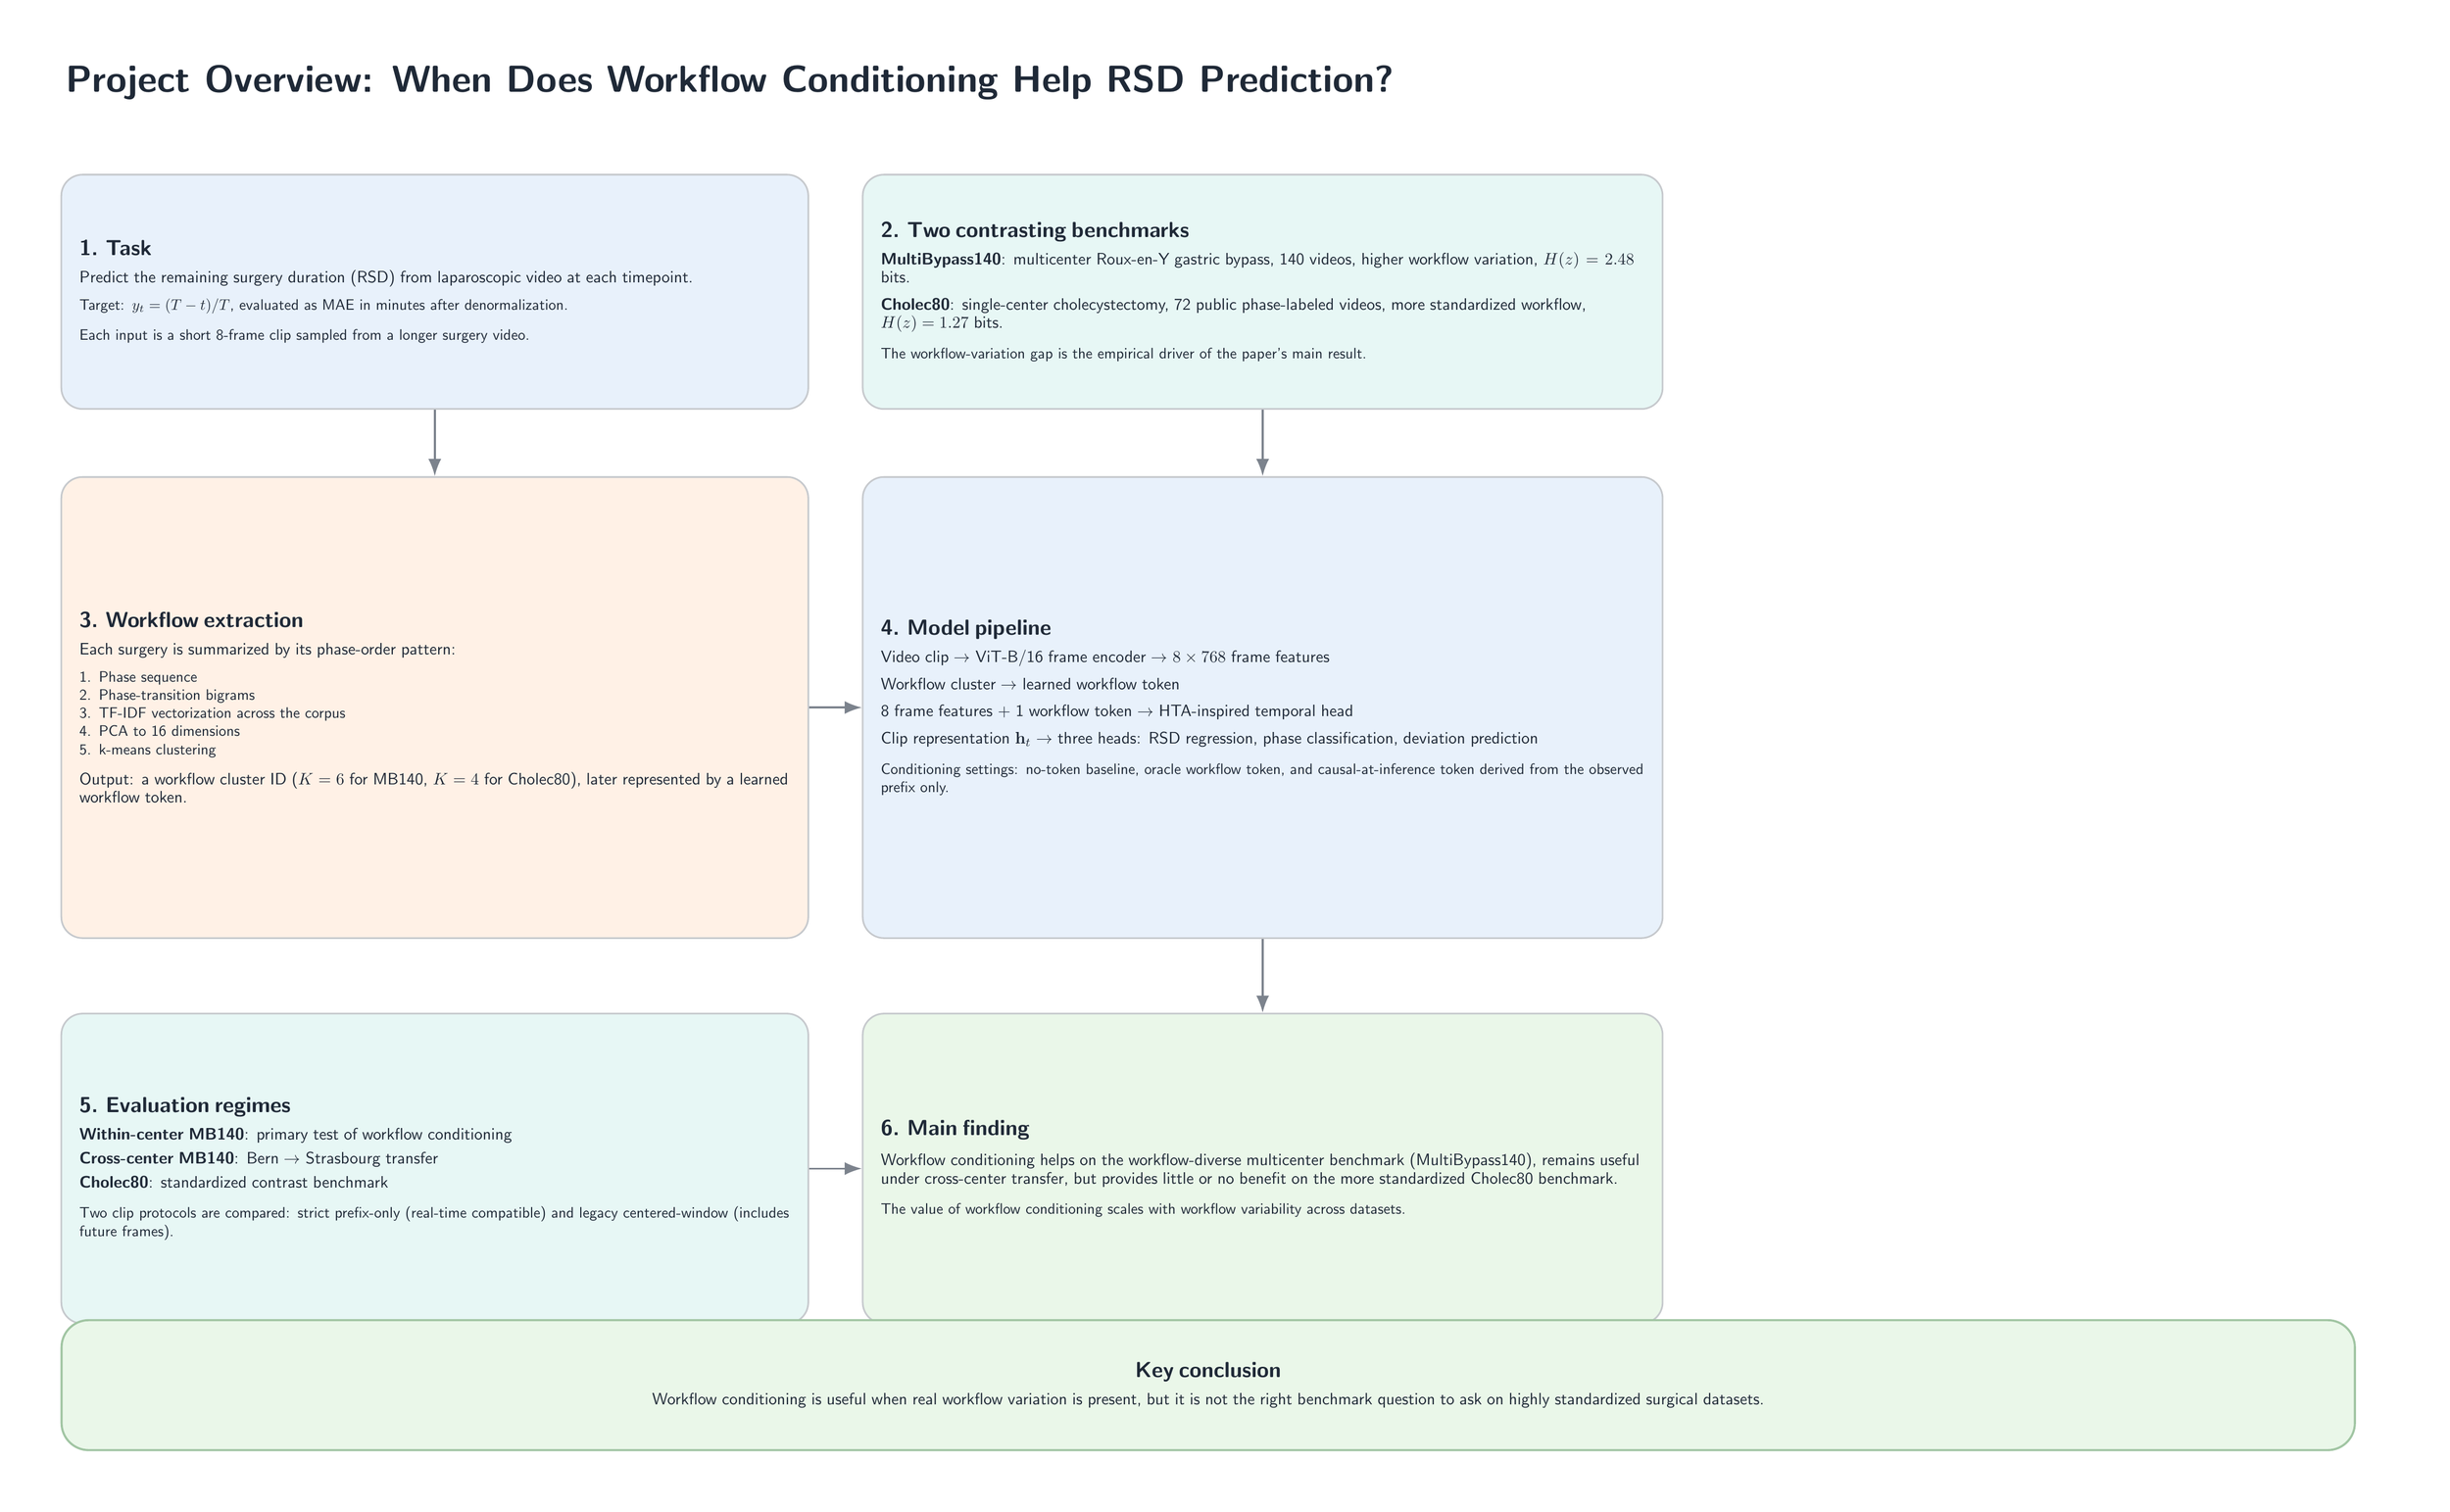
\begin{tikzpicture}[x=1pt,y=1pt]
\useasboundingbox (0,0) rectangle (1600,980);

\node[title, anchor=north west] at (30,950)
{Project Overview: When Does Workflow Conditioning Help RSD Prediction?};

\node[bluebox, text width=470pt, minimum height=155pt, anchor=north west] (task) at (30,875) {
{\subtitle 1. Task}\par\vspace{6pt}
{\body Predict the remaining surgery duration (RSD) from laparoscopic video at each timepoint.}\par\vspace{6pt}
{\smallbody Target: \(y_t = (T - t)/T\), evaluated as MAE in minutes after denormalization.}\par\vspace{8pt}
{\smallbody Each input is a short 8-frame clip sampled from a longer surgery video.}
};

\node[tealbox, text width=505pt, minimum height=155pt, anchor=north west] (bench) at (560,875) {
{\subtitle 2. Two contrasting benchmarks}\par\vspace{6pt}
{\body \textbf{MultiBypass140}: multicenter Roux-en-Y gastric bypass, 140 videos, higher workflow variation, \(H(z)=2.48\) bits.}\par\vspace{6pt}
{\body \textbf{Cholec80}: single-center cholecystectomy, 72 public phase-labeled videos, more standardized workflow, \(H(z)=1.27\) bits.}\par\vspace{8pt}
{\smallbody The workflow-variation gap is the empirical driver of the paper's main result.}
};

\node[orangebox, text width=470pt, minimum height=305pt, anchor=north west] (workflow) at (30,675) {
{\subtitle 3. Workflow extraction}\par\vspace{6pt}
{\body Each surgery is summarized by its phase-order pattern:}\par\vspace{6pt}
{\smallbody 1. Phase sequence}\par
{\smallbody 2. Phase-transition bigrams}\par
{\smallbody 3. TF-IDF vectorization across the corpus}\par
{\smallbody 4. PCA to 16 dimensions}\par
{\smallbody 5. k-means clustering}\par\vspace{8pt}
{\body Output: a workflow cluster ID (\(K=6\) for MB140, \(K=4\) for Cholec80), later represented by a learned workflow token.}
};

\node[bluebox, text width=505pt, minimum height=305pt, anchor=north west] (model) at (560,675) {
{\subtitle 4. Model pipeline}\par\vspace{6pt}
{\body Video clip \(\rightarrow\) ViT-B/16 frame encoder \(\rightarrow\) \(8\times768\) frame features}\par\vspace{6pt}
{\body Workflow cluster \(\rightarrow\) learned workflow token}\par\vspace{6pt}
{\body 8 frame features + 1 workflow token \(\rightarrow\) HTA-inspired temporal head}\par\vspace{6pt}
{\body Clip representation \(\mathbf{h}_t\) \(\rightarrow\) three heads: RSD regression, phase classification, deviation prediction}\par\vspace{8pt}
{\smallbody Conditioning settings: no-token baseline, oracle workflow token, and causal-at-inference token derived from the observed prefix only.}
};

\node[tealbox, text width=470pt, minimum height=205pt, anchor=north west] (eval) at (30,320) {
{\subtitle 5. Evaluation regimes}\par\vspace{6pt}
{\body \textbf{Within-center MB140}: primary test of workflow conditioning}\par\vspace{4pt}
{\body \textbf{Cross-center MB140}: Bern \(\rightarrow\) Strasbourg transfer}\par\vspace{4pt}
{\body \textbf{Cholec80}: standardized contrast benchmark}\par\vspace{8pt}
{\smallbody Two clip protocols are compared: strict prefix-only (real-time compatible) and legacy centered-window (includes future frames).}
};

\node[greenbox, text width=505pt, minimum height=205pt, anchor=north west] (find) at (560,320) {
{\subtitle 6. Main finding}\par\vspace{8pt}
{\body Workflow conditioning helps on the workflow-diverse multicenter benchmark (MultiBypass140), remains useful under cross-center transfer, but provides little or no benefit on the more standardized Cholec80 benchmark.}\par\vspace{8pt}
{\smallbody The value of workflow conditioning scales with workflow variability across datasets.}
};

\draw[arrow] (task.south) -- ++(0,-18) -| (workflow.north);
\draw[arrow] (bench.south) -- ++(0,-18) -| (model.north);
\draw[arrow] (workflow.east) -- ++(18,0) |- (model.west);
\draw[arrow] (model.south) -- ++(0,-18) -| (find.north);
\draw[arrow] (eval.east) -- ++(18,0) -- (find.west);

\node[rounded corners=18pt, draw=greenB!45, fill=greenA, line width=1.4pt, text width=1510pt, minimum height=86pt, align=center, anchor=south west] at (30,30) {
{\subtitle Key conclusion}\par\vspace{6pt}
{\body Workflow conditioning is useful when real workflow variation is present, but it is not the right benchmark question to ask on highly standardized surgical datasets.}
};

\end{tikzpicture}
\end{document}
